\chapter{Theoretical Background}
\label{chap:theoretical-background}
This chapter provides an overview of the technologies and concepts referred to in subsequent chapters.
Starting with section \ref{sec:computer-networks}, essential concepts of computer communication in networks will be presented and examined, covering the concept of network layers, intercepting of communication between two parties and analysis of transferred data.
Building upon these fundamentals, section \ref{sec:internet-of-things} introduces the fields of use of \ac{IoT} applications, common architectures used today to implement them and popular protocols they make use of. Lastly, it will discuss security considerations important to \ac{IoT} applications.
After that, section \ref{sec:information-security} will provide insights into relevant concepts and the practices used and applied in information security. It covers key concepts and legal considerations, integration of information security in software development and common practices and methods involved. %TODO: Update


\section{Design Patterns}
The following sub-sections introduce a set of design patterns that are of relevance to this work.

\subsection{Pipeline/Pipes and Filters Pattern}
In a paper from 1996, Alencar et al. describe the pipes and filters pattern as a mechanism to process streams of data \cite{alencar_cowan_lucena_1996}. They state that the pattern features \enquote{pipes} and \enquote{filters} components: pipes relay data streams between filters while the filters process the data streams' contents. Figure \ref{fig:dp-pipes-filters} shows an exemplaric sequence of $n$ pipes and filters relaying and processing an object $O$ by implementing pipes as method calls. Alencar et al. state that the pattern's \enquote{objective is to obtain highly reusable, interchangeable and maintainable applications}.
\begin{figure}[h!]
    \centering
    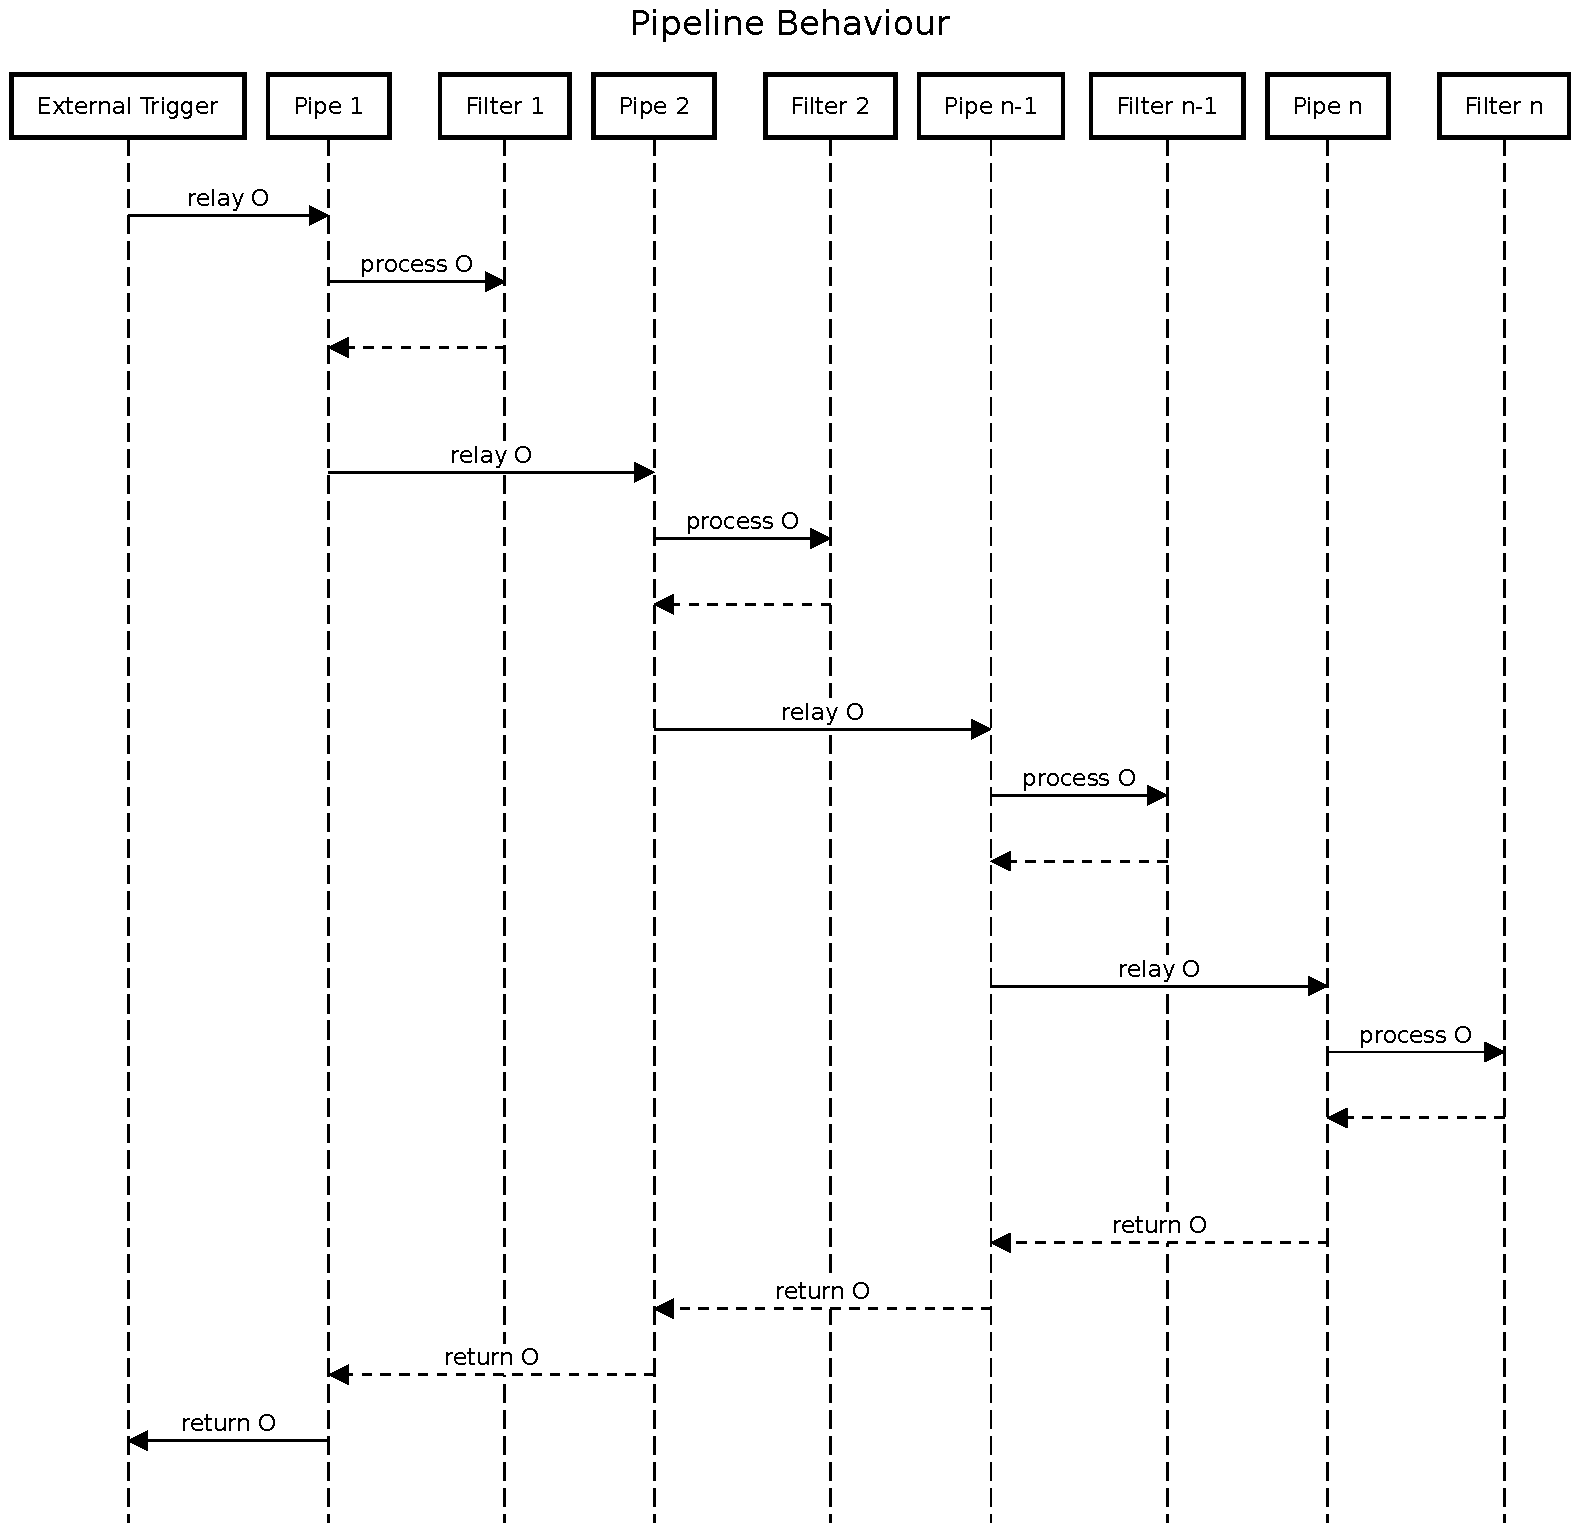
\includegraphics[width=14cm]{img/ch03/pipeline-behaviour.pdf}
    \captionof{figure}{?} % TODO: Describe
    \label{fig:dp-pipes-filters}
\end{figure}
\subsection{Abstract Factory/Kit Pattern}
Gamma et al. describe the intent of the abstract factory pattern as follows: "provide an interface for creating families of related or dependent objects without specifying their concrete classes" \cite{Gamma1998}. They propose the following components:
\begin{itemize}
    \item \enquote{AbstractProduct}: interface for products.
    \item \enquote{AbstractFactory}: interface for creating objects that implement \enquote{AbstractProduct}.
    \item \enquote{ConcreteProduct}: classes that implement \enquote{AbstractProduct}.
    \item \enquote{ConcreteFactory}: classes that implements \enquote{AbstractFactory} and create \enquote{ConcreteProducts}.
    \item \enquote{Client}: class that only uses the interfaces of \enquote{AbstractProducts} and \enquote{AbstractFactories}.
\end{itemize}
They conclude that there are multiple consequences to using the pattern, one being that it \enquote{isolates concrete classes}, meaning that there is a clear isolation from the Client and the ConcreteFactories.
%CITE: 1996 Paper Design Patterns in Software Design Patterns
%CITE: 1997 - Book - Design Patterns
\subsection{Publish-Subscribe/Observer Pattern}
%CITE: 1997 - Book - Design Patterns
In their book \enquote{Design Patterns - Elements of Reusable Object-oriented Software}, Gamma et al. state that the observer pattern aims to "define a one-to-many dependency between objects so that when one object changes state, all its dependents are notified and updated automatically" \cite{Gamma1998}. To achieve this, they propose the following components:
\begin{itemize}
    \item \enquote{Observer}: interface for observing objects. It defines a single \emph{Update} method.
    \item \enquote{Subject}: interface for observable objects that can (un-)register \enquote{Observers} by defining \emph{Attach} and \emph{Detach} methods. It can notify its registered \enquote{Observers} by use of its \emph{Notify} method which calls all of its \enquote{Observers'} \emph{Update} methods.
\end{itemize}
Gamma et al. point out a number of benefits using this pattern. The \enquote{support for broadcast communication} is a benefit of particular relevance for this thesis as it puts a focus on the simplification of the process of sending notification to multiple, interested objects. For this reason, this pattern is used in communication protocols such as \ac{MQTT} (further elaborated on in section \ref{sec:iot-common-protocols}).


\section{Computer Communication: The OSI-Model}
\label{sec:computer-networks}
The \ac{OSI}-Model was initially proposed in the \ac{ISO}/\ac{IEC} standard \enquote{\ac{ISO} 7498 - Information processing systems — Open Systems Interconnection — Basic Reference Model} in 1984 and revised in 1994 by the \ac{ISO}/\ac{IEC} standard 7498-1 \cite{ISOIEC74981}. It aims to formalize a unified approach to communication between diverse peer systems by defining the \emph{network layers} shown in figure \ref{fig:osi-model}. These layers are read from bottom to top, increasing in complexity and abstraction:
\begin{figure}[h!]
    \centering
    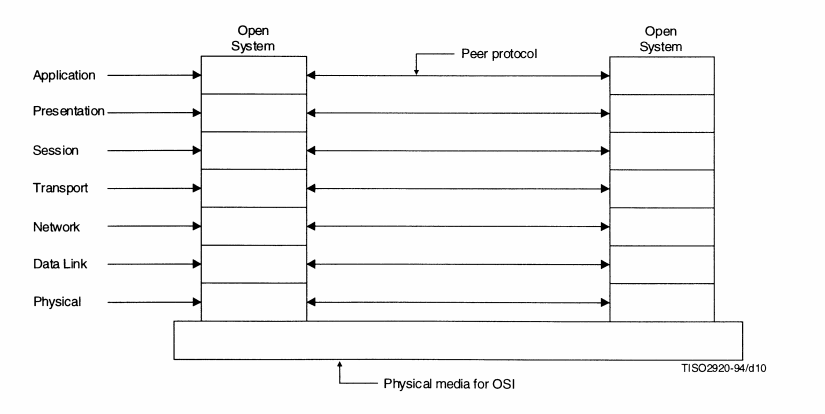
\includegraphics[width=14cm]{img/ch03/osi-model.png}
    \captionof{figure}{\enquote{Seven layer reference model and peer protocols} \cite{ISOIEC74981} as proposed in \ac{ISO}/\ac{IEC} 7498.}
    \label{fig:osi-model}
\end{figure}
\begin{enumerate}
    \item Physical: Bitwise transmission of data (e.g. via copper cable or fibre glass).
    \item Data Link: Aggregation of bitwise data into data frames (e.g. via Ethernet packets sent via \ac{WLAN}) and transmission of those frames to a communication destination.
    \item Network: Encapsulates data frames into packets (e.g. \ac{IP} packets) and routes and relays those packets across network nodes that are identified by addresses (i.e. \ac{IP} addresses).
    \item Transport: Splits packets of arbitrary lengths into transmissible packets and ensures their successful transmission (when using \ac{TCP}). Also, it servers as an abstraction layer for applications that operate on higher layers.
    \item Session: Nowadays part of the \ac{TCP} protocol, the session layer handles establishing and terminating of connections between applications.
    \item Presentation: Encoding information in a format accepted by all communication peers involved (i.e. \ac{XML} and \ac{JSON}).
    \item Application: High-level application functionality that makes use of the lower layers to communicate with peers (e.g. \ac{HTTP}).
\end{enumerate}
This concept of a stack of network layers results in a series of encapsulated messages. For example, a large \ac{HTTP} response containing a binary file can be represented as follows over the various layers:
\begin{etaremune}
    \item Application: The \ac{HTTP} response itself.
    \item Presentation: The text-based \ac{HTTP} headers and the binary content encoded as raw bytes.
    \item \textit{(Session: Part of the \ac{TCP} protocol.)}
    \item Transport: Multiple \ac{TCP} packets with a binary payload and header information about the source and destination ports.
    \item Network: Multiple \ac{IP} packets with a binary payload and header information about the source and destination addresses.
    \item Data Link: Multiple Ethernet frames with a binary payload and header information about the source and destination peer's \ac{MAC} addresses.
    \item \textit{(Physical: Stream of individual bits that make up the Ethernet frames.)}
\end{etaremune}


\section{Internet of Things}
\label{sec:internet-of-things}
\subsection{Fields of Use}
In their paper, Perera et al. categorized \ac{IoT} applications into several classes \cite{IOTSurvey}:
\begin{itemize}
    \item[A]{Smart Wearable: smart products that can be worn on different body parts or clothing.}
    \item[B]{Smart Home: connected applications installed and/or used in home environments.}
    \item[C]{Smart City: connected applications for large-scale use in cities that support logistic challenges such as traffic control and resource management.}
    \item[D]{Smart Environment: applications that provide monitoring capabilities for environmental metrics such as air quality and water quality.}
    \item[E]{Smart Enterprise: applications used in commercial and industrial environments to address challenging tasks such as logistics, transportation and energy management.}
\end{itemize}

\subsection{Common Protocols}
\label{sec:iot-common-protocols}
Building up on pre-existing network infrastructure and in order to meet requirements specific to individual fields of use and use-case scenarios, the landscape of \ac{IoT} attends with a great variety of \emph{communication protocols} (further used to refer to both transport and application protocols). This section will provide a brief overview of the working principles, use cases and history of some protocols commonly used in \ac{IoT} and \ac{IIoT} applications today.
\paragraph{\ac{HTTP}}
Initially conceived by Berners-Lee et al. at the \ac{CERN} in 1991, the \ac{HTTP} protocol is an application layer protocol that defines \emph{requests} to resources made by clients and \emph{responses} to said requests replied by servers \cite{http1991}. According to RFC1945, \ac{HTTP} requests consist of \cite{rfc1945}:
\begin{itemize}
    \item A request line including the \ac{HTTP} verb (e.g. $GET$ or $POST$), the requested resource and the \ac{HTTP} version used (e.g. $HTTP/1.0$). The verb can be used to indicates what kind action is requested (i.e. a $GET$ request should retrieve contents while a $POST$ request could be used to create new content). The request line is terminated by a set of \ac{CR} \ac{LF} characters.
    \item A set of request header fields delimited by a set of \ac{CR} \ac{LF} characters where headers are encoded in the format $Key: Value$.
    \item An empty line indicates the end of the header fields.
    \item Optionally, requests can contain a message body. Its encoding is dependent on value of the $Content-Type$ header. If present, the length of the message body is specified in the $Content-Length$ header.
\end{itemize}
The structure of \ac{HTTP} responses is similar to \ac{HTTP} requests \cite{rfc1945}:
\begin{itemize}
    \item A status line including the \ac{HTTP} version and status code (e.g. $200$ meaning \enquote{OK}, indicating a successful response). The status line is terminated by a set of \ac{CR} \ac{LF} characters.
    \item A set of response header fields, encoded just like the above-said request headers.
    \item An empty line.
    \item Optional message body. Like request message bodies, the encoding of the message body depends on the value of the $Content-Type$ header.
\end{itemize}
Figure \ref{fig:curl-http-request-respose} shows a \ac{HTTP} requests to the site \enquote{httpbin.org}. By definition, \ac{HTTP} sends data in clear-text. Thus, \ac{HTTP} communication can be intercepted and manipulated by malicious actors. \ac{HTTPS} was introduced to solve this issue by sending \ac{HTTP} requests and responses through \ac{SSL} encrypted connections \cite{rfc2818}.

\begin{figure}[h!]
    \centering
    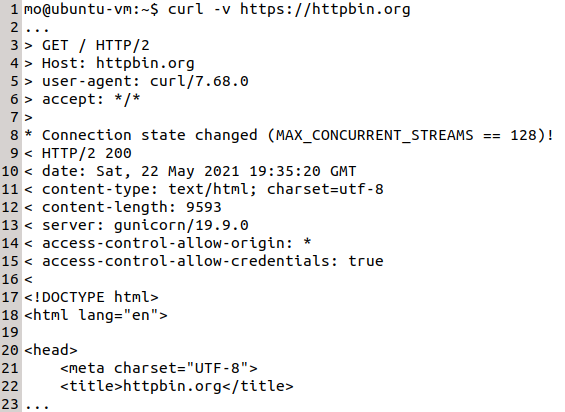
\includegraphics[width=12cm]{img/ch03/http-request-response.png}
    \captionof{figure}{A truncated \ac{HTTP} request (indicated by \enquote{>}) to \enquote{httpbin.org} using the utility \enquote{curl} and the truncated response received from the remote server (indicated by \enquote{<}).} %TODO: Describe
    \label{fig:curl-http-request-respose}
\end{figure}

%CITE: 1.0 https://datatracker.ietf.org/doc/html/rfc1945
%CITE: 2019 - Book - SmartInnovationsInCommunicatio - p174
\paragraph{\ac{WS}} \emph{TBD}

%CITE: https://datatracker.ietf.org/doc/html/rfc6455
%CITE: PMCE https://tools.ietf.org/html/rfc7692
\paragraph{\ac{MQTT}}
\cite{gupta_banks_2015}

\paragraph{Industrial} Modbus \ac{TCP}, Profibus/Profinet, \ac{OPC U/A}

\section{Information Security}
\label{sec:information-security}
\subsection{The CIA Triad}

\subsection{Methodology}
\subsubsection{Penetration Testing}
\subsubsection{Red-Teaming}
\subsubsection{Fuzzing}

\subsection{Man-In-The-Middle Attacks}
\ac{MITM}
%Cite: A Survey of Man In The Middle Attacks

\subsection{Tools}
There are many tools used in information security. They vary greatly in their features, field of use and maturity. The following paragraphs describe tools relevant to this thesis and the fields of use it touches.

\paragraph{Wireshark} First released in 1998, \emph{Wireshark} is a cross-platform and open-source tool used for network analysis, including \emph{network sniffing} \cite{wireshark}. It is written mainly in C, consists of more than 3,600,000 lines of C code\footnote{This number was returned by the \emph{cloc} utility run on commit \emph{c73ab16b} from 23rd May 2021 of Wireshark's GitLab source-code repository \cite{wiresharkgit}.} and features a \ac{GUI}. Although it is described as a network protocol analyser, it also supports sniffing of \ac{USB} packets. It implements a wide array of \emph{dissectors} for various protocols and allows detailed examination of network packets (as shown in figure \ref{fig:wireshark}).

\begin{figure}[h]
    \centering
    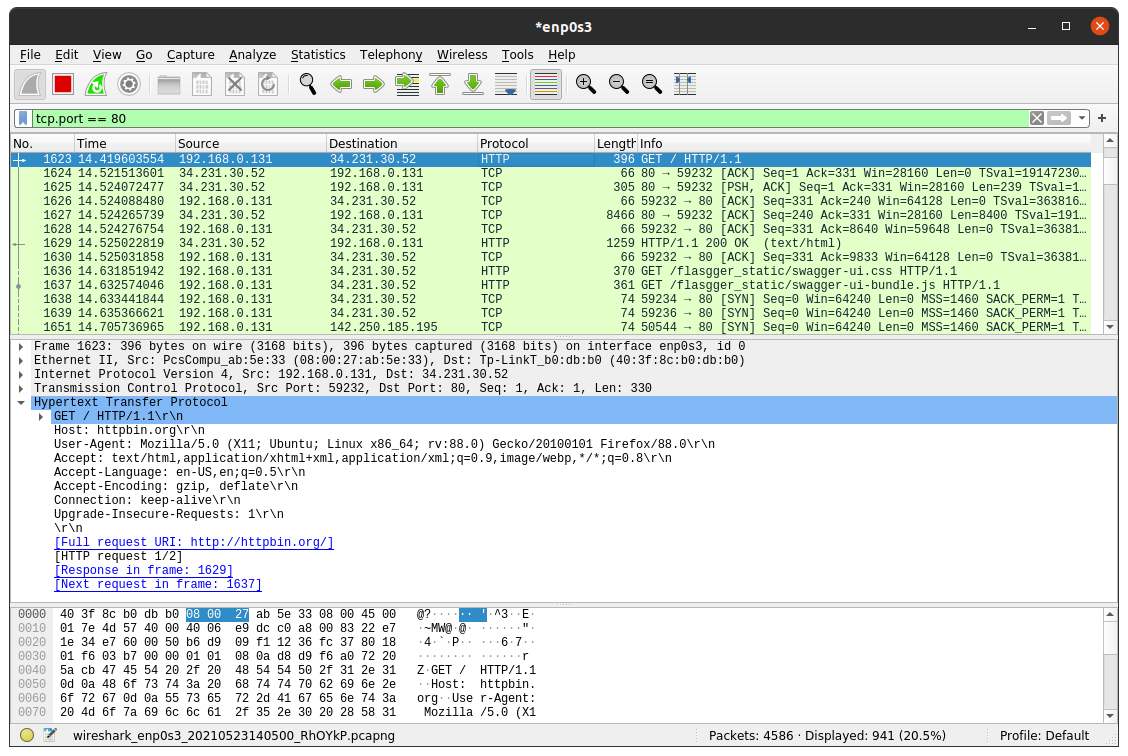
\includegraphics[width=14cm]{img/ch03/wireshark.png}
    \captionof{figure}{Screenshot of Wireshark being executed and dissecting a \ac{HTTP} $GET$ request to the site \enquote{httpbin.org}. The display-filter \enquote{tcp.port == 80} shows only packets sent to or from port 80 (e.g. \ac{HTTP} communication).}
    \label{fig:wireshark}
\end{figure}

\subsubsection{Specific \acp{MITM}}
The following tools are \acp{MITM} that support specific protocols only:
%Specific mitms:
\paragraph{Burp Suite} Developed and distributed by \enquote{PortSwigger} as a commercial product, \emph{Burp Suite} is a tool specialized for web-application testing \cite{burpsuite}. It can be used as a \ac{MITM} for \ac{HTTP} communication by configuring the operating system or browser to use its internal \ac{HTTP} server as a proxy. While it implements basic support for \ac{WS}, it is mainly used for \ac{HTTP} (and nowadays \ac{HTTPS}) and lacks support for other protocols. Aside from its internal proxy server, it also provides specialized features such as the \enquote{Repeater} which is used to send forged \ac{HTTP} requests. The freely available \enquote{Community Edition} (shown in figure \ref{fig:burpsuite}) allows use of most of the tool's features.

\begin{figure}[h]
    \centering
    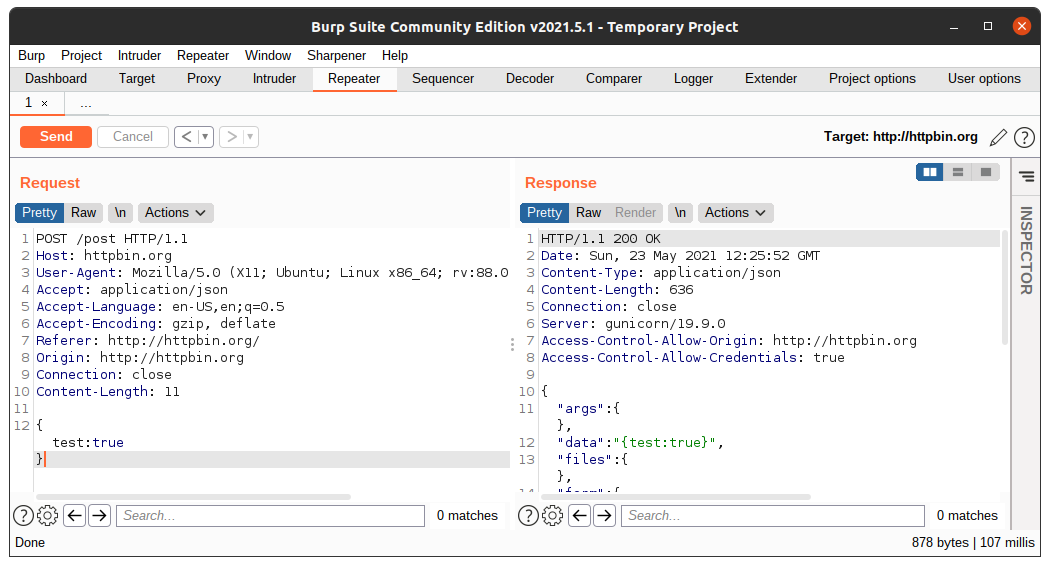
\includegraphics[width=14cm]{img/ch03/burpsuite.png}
    \captionof{figure}{Screenshot of Burp Suite being used to send forged \ac{HTTP} requests to the site \enquote{httpbin.org}.}
    \label{fig:burpsuite}
\end{figure}
\paragraph{mitmproxy} %focused on HTTP/S + WS but supports extension, largely undocumented source
\paragraph{mProxy}
\paragraph{IOXY}
%Generic
\subsubsection{Generic \acp{MITM}}
The following tools are generic \acp{MITM} that support a wide range of network protocols:
\paragraph{ettercap} While \emph{ettercap} was initially developed as a network sniffer for switched \ac{LAN}, it was gradually extended to implement a set of \ac{MITM} attacks such as \ac{ARP} spoofing and \emph{packet filtering} which allowed modifying intercepted communication \cite{ettercap}. Penetration testers can write custom filters in a scripting language to implement their own packet filtering logic. It is written in C and implements network protocols of layers 1 to 4 of the \ac{OSI} model. Thus, it does not implement application protocols.
\paragraph{bettercap} Similar to ettercap, \emph{bettercap} implements network sniffing and other features used for network analysis and discovery. However, contrary to ettercap, it aims to support a wider range of transport technologies and is described as \enquote{\emph{the Swiss Army knife for WiFi, Bluetooth Low Energy, wireless HID hijacking and IPv4 and IPv6 network reconnaissance and MITM attacks}} \cite{bettercap}. It is written in Go and features a web-interface for configuration, control and monitoring.
\paragraph{Scapy}
\paragraph{MITMf} %Built on scapy, implements some attacks and servers, not maintained anymore, superseded by bettercap 